\documentclass[titlepage,12pt]{article}

% Imported Packages
%------------------------------------------------------------------------------
\usepackage{amssymb}
\usepackage{amstext}
\usepackage{amsthm}
\usepackage{amsmath}
\usepackage{enumerate}
\usepackage{fancyhdr}
\usepackage[margin=1in]{geometry}
\usepackage{graphicx}
\usepackage{extarrows}
\usepackage{setspace}

\usepackage{array}
\usepackage{color}
\usepackage[hidelinks]{hyperref}
\usepackage{float}
%------------------------------------------------------------------------------

% Custom commands
%------------------------------------------------------------------------------
\newcounter{myCounter}

%------------------------------------------------------------------------------

% Header and Footer
%------------------------------------------------------------------------------
\pagestyle{plain}
\renewcommand\headrulewidth{0.4pt}
\renewcommand\footrulewidth{0.4pt}
%------------------------------------------------------------------------------

% Title Details
%------------------------------------------------------------------------------
\title{ParkFinder\\Software Requirements Document\\SE 3A04}
\author{Abdul Ahad \\ akhteraa \and Salma Belal \\ belalsm \and Josh Chatten \\ chattejj \and
Nathanael Jordan \\ jordanen \and Robert Stuart \\ stuarr2}
\date{\today}

%------------------------------------------------------------------------------

% Document
%------------------------------------------------------------------------------
\begin{document}

\maketitle	
\thispagestyle{empty}
\clearpage
\setcounter{tocdepth}{2}% Only show down to subsections?
\tableofcontents
\clearpage

\section{Introduction}
\label{sec:introduction}
% Begin Section

%This section should provide an brief overview of the entire document.

\subsection{Purpose}
\label{sub:purpose}
% Begin SubSection

The purpose of this Design Document is to provide a description for the design of the Park Finder
app. The description of the design will allow anyone who will be involved in the development of the
system to proceed with an understanding of what is to be built and how it is expected to be built.
This document provides a description of the system architecture, as well as diagrams that model the
functionality of system, describe the key classes of the system, their interrelationship, and their
responsibilities.

The intended readers of this document include all of the project's stakeholders. This includes the
end-user, the software engineers, and the park authorities.

% End SubSection

\subsection{System Description}
\label{sub:system_description}
%Begin SubSection

The software system being described in this document is called the ParkFinder app. This system will
have datasets of information about parks from all over the world and will allow the client to use
search methods in order to find parks based on the clients' desired attributes. The app is meant to
be used anywhere in the world, provided an Android or iOS device with the app installed. This
provides clients with an easier, faster, and more efficient way to look up parks and acquire
information such as the location, facilities, activities, and rentals that the parks provide.

% End SubSection

\subsection{Overview}
\label{sub:overview}
% Begin SubSection

The remainder of this document will contain diagrams and information that will describe the details
for the software system being built. This will include a use case diagram in Section~
\ref{sec:use_case_diagram}, an analysis class diagram in Section~\ref{sec:analysis_class_diagram}, a
description of the architectural design in Section~\ref{sec:architectural_design}, and CRC cards for
all identified classes in Section~\ref{sec:class_responsibility_collaboration_crc_cards}.

% End SubSection

% End Section

\section{Use Case Diagram}
\label{sec:use_case_diagram}
% Begin Section

%This section should provide a use case diagram for your application. 
%\begin{enumerate}[a)]
%    \item Each use case appearing in the diagram should be accompanied by a text description. 
%\end{enumerate}

\begin{figure}[htbp]
\centerline{\includegraphics[width=0.9\textwidth]{images//UseCase}}
\caption{Use Case Diagram}
\label{useCaseDiagram}
\end{figure}

\begin{enumerate}[a)]
    \item \textbf{Search for parks:} The user searches for parks. This is accomplished by consulting
    experts based on which park attributes were selected by the user.
    \item \textbf{Browse park's listing} User browses a list of parks, this list can either be the
    result of a previous search action or a default list (all parks).
    \item \textbf{Select park(s):} User selects a park or several parks from the list they were
    browsing, this displays addition park information to the user as well as the park(s) on a map if
    desired.
    \item \textbf{Request nearest 5 parks:} User requests the five nearest parks to their current
    location. \textcolor{red}{should request nearest 5 parks be linked to browse park listing?}
    \item \textbf{Swap or remove expert:} A developer attempts to swap or remove an expert from the
    system, the system requires authorization from a manager for the change to occur.
    \item \textbf{Authorize expert modification:} \textcolor{red}{is this a use case? or part of the
    swap/remove use case?}
\end{enumerate}

% End Section

\section{Analysis Class Diagram}
\label{sec:analysis_class_diagram}
% Begin Section

\begin{figure}[H]
	\centerline{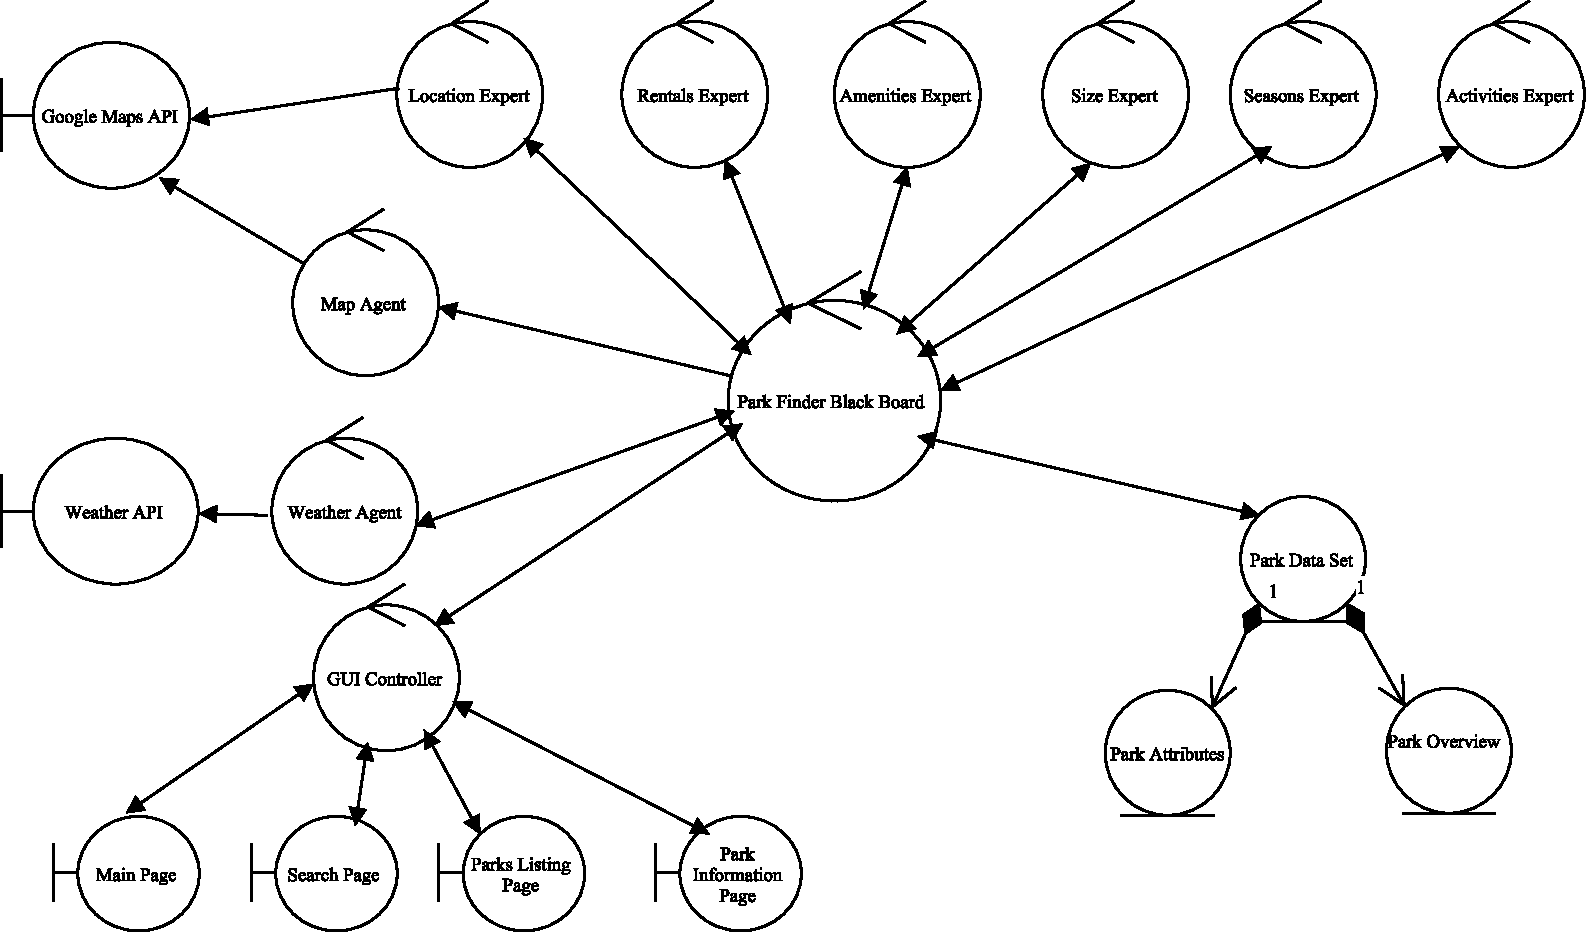
\includegraphics[width=0.9\textwidth]{images//analysis_class_diagram}}
	\caption{Analysis Class Diagram}
	\label{analysisClassDiagram}
\end{figure}

% End Section

\section{Architectural Design}
\label{sec:architectural_design}
% Begin Section

%This section should provide an overview of the overall architectural design of your application.
%Your overall architecture should show the division of the system into subsystems with high
%cohesion and low coupling.

\subsection{System Architecture}
\label{sub:system_architecture}
% Begin SubSection

%\begin{enumerate}[a)]
%    \item Identify and explain the overall architecture of your system
%    \item Be sure to clearly state the name of the architecture
%    \item Provide the reasoning and justification of the choice
%    \item Provide a structural architecture diagram showing the relationship among the subsystems
%    (if appropriate)
%\end{enumerate}

% End SubSection

\subsection{Subsystems}
\label{sub:subsystems}
% Begin SubSection

The system will be divided into several different subsystems that are shown in Figure~
\ref{analysisClassDiagram}. Each of these subsystems will handle different functionality of the
overall system. The GUI and User subsystems will handle all interactions with the user of the
application. The database will contain all of the information about each park in the system. The
several Expert subsystems will have similar functionality but handle different information. Each
Expert subsystem will be provided search criteria and will return all parks which satisfy the
criteria. The Weather Agent will provide the weather at any requested location. Lastly, ParkFinder
will handle the information flow between all of the subsystems. ParkFinder will receive the user
search criteria from GUI then provide that information and the database to the appropriate Expert(s)
in order to identify the correct park.

% End SubSection

% End Section
    
\section{Class Responsibility Collaboration (CRC) Cards}
\label{sec:class_responsibility_collaboration_crc_cards}
% Begin Section

%This section should contain all of your CRC cards.
%
%\begin{enumerate}[a)]
%    \item Provide a CRC Card for each identified class
%    \item Please use the format outlined in tutorial, i.e., 
%    \begin{table}[ht]
%        \centering
%        \begin{tabular}{|p{5cm}|p{5cm}|}
%        \hline 
%        \multicolumn{2}{|l|}{\textbf{Class Name:}} \\
%        \hline
%        \textbf{Responsibility:} & \textbf{Collaborators:} \\
%        \hline
%        \vspace{1in} & \\
%        \hline
%        \end{tabular}
%    \end{table}
%    
%\end{enumerate}

% End Section

\newpage
\appendix
\section{Division of Labour}%TODO
\label{sec:division_of_labour}
% Begin Section

\begin{table}[htbp]
\vspace{-0.06in}
\begin{center}
\setlength{\extrarowheight}{4.0pt}
\begin{tabular}{m{0.3\textwidth} m{0.2\textwidth} m{0.3\textwidth}} 
\hline
\textbf{Contributions} & \textbf{Name} & \textbf{Signature}\\
\hline
x & Abdul Ahad & \\
\hline
x & Salma Belal & \\
\hline
x & Josh Chatten & \\
\hline
x & Nathanael Jordan  & \\
\hline
x & Robert Stuart & \\
\hline
\end{tabular}
\end{center}
\label{divOfLabour}
\end{table}

% End Section

\newpage
\section*{IMPORTANT NOTES}
\begin{itemize}
%   \item You do \underline{NOT} need to provide a text explanation of each diagram; the diagram
% should speak for itself
    \item Please document any non-standard notations that you may have used
    \begin{itemize}
        \item \emph{Rule of Thumb}: if you feel there is any doubt surrounding the meaning of your
        notations, document them
    \end{itemize}
    \item Some diagrams may be difficult to fit into one page
    \begin{itemize}
        \item It is OK if the text is small but please ensure that it is readable when printed
        \item If you need to break a diagram onto multiple pages, please adopt a system of doing so
        and thoroughly explain how it can be reconnected from one page to the next; if you are
        unsure about this, please ask about it
    \end{itemize}
    \item Please submit the latest version of Deliverable 1 with Deliverable 2
    \begin{itemize}
        \item It does not have to be a freshly printed version; the latest marked version is OK
    \end{itemize}
    \item If you do \underline{NOT} have a Division of Labour sheet, your deliverable will
    \underline{NOT} be marked
\end{itemize}

\end{document}
%------------------------------------------------------------------------------